\documentclass[letterpaper,10pt]{article}
\usepackage{graphicx}
\usepackage{listings}
\usepackage{fullpage}
\usepackage{fixltx2e}
\usepackage{multirow}
\usepackage{amssymb,amsmath}
\usepackage{mathtools}
\usepackage{bm}
\usepackage[hyperfootnotes=false]{hyperref}
\usepackage{url}
\usepackage{subfig}
\usepackage{relsize}
\usepackage{enumitem}
\usepackage{fancyhdr}
\usepackage{framed}
\setlength{\headheight}{14pt}
\pagestyle{fancy}
\headsep = 20pt

% Lineskip mods
\linespread{1.0}
\setlength{\parskip}{0.5\baselineskip}
\setlength{\parindent}{0pt}
\newlength\docparskip
\parskip=6pt
\setlength{\docparskip}{\parskip}
\renewcommand{\arraystretch}{1.085}
\usepackage{xcolor}
\lstset{basicstyle=\ttfamily,
  showstringspaces=false,
  commentstyle=\color{red},
  keywordstyle=\color{blue}
}
\begin{document}

\fancyhf{}
\fancyhead[L]{AME 60614: Numerical Methods}
\fancyhead[R]{Qihao Zhuo: Problem Set 3}
\fancyfoot[C]{\thepage}

\thispagestyle{plain}
\begin{center}
  \large
  \textbf{AME 60614: Numerical Methods} \\
  \textbf{Fall 2021} \\
  \vspace{0.5em}
  \textbf{Problem Set 3} \\
  \vspace{1em}
  Qihao Zhuo
\end{center}

\vspace{1.5em}

\section{Modified Wavenumber Analysis}\label{sec1}
\begin{align*}
  \frac{\partial \phi}{\partial t}&=\alpha \frac{\partial^2 \phi}{\partial x^2}\\
  \phi_j &= \psi(t)e^{ikx_j}\\
  \frac{d\psi}{dt}&=-\alpha k^2 \phi
\end{align*}

Considering the second-order one-sided scheme, 
\begin{align*}
  \frac{d\phi_j}{dt}&=\frac{\alpha}{\Delta x^2}\left(-\phi_{j+3}+4\phi_{j+2}-5\phi_{j+1}+2\phi_j\right)\\
  &=\frac{\alpha}{\Delta x^2}\left(-\psi e^{ikx_j}e^{ik3\Delta x}+4\psi e^{ikx_j}e^{ik2\Delta x}-5\psi e^{ikx_j}e^{ik\Delta x}+2\psi e^{ikx_j}\right)\\
  &=\frac{\alpha \phi}{\Delta x^2}\left(-e^{ik3\Delta x}+4e^{ik2\Delta x}-5e^{ik\Delta x}+2\right)\\
  &=\frac{\alpha \phi}{\Delta x^2}\left(-\cos 3\Delta x-i\sin 3\Delta x+4\cos 2\Delta x +4i\sin 2\Delta x - 5\cos \Delta x -5i\sin \Delta x +2\right)\\
  &=\frac{\alpha}{\Delta x^2}\left[\left(2-\cos3\Delta x+4\cos 2\Delta x-5\cos \Delta x\right)-i\left(\sin 3\Delta x -4\sin 2\Delta x - 5\sin \Delta x\right)\right]\phi\\
  &=-\frac{\alpha}{\Delta x^2}\left[\left(-2+\cos3\Delta x-4\cos 2\Delta x+5\cos \Delta x\right)+i\left(\sin 3\Delta x -4\sin 2\Delta x - 5\sin \Delta x\right)\right]\phi\\
  -\alpha k^{'2} \phi &=-\frac{\alpha}{\Delta x^2}\left[\left(-2+\cos3\Delta x-4\cos 2\Delta x+5\cos \Delta x\right)+i\left(\sin 3\Delta x -4\sin 2\Delta x - 5\sin \Delta x\right)\right]\phi\\
  -\alpha k^{'2} &=-\frac{\alpha}{\Delta x^2}\left[\left(-2+\cos3\Delta x-4\cos 2\Delta x+5\cos \Delta x\right)+i\left(\sin 3\Delta x -4\sin 2\Delta x - 5\sin \Delta x\right)\right]\\
  k^{'2}&=\frac{1}{\Delta x^2}\left[\left(-2+\cos3\Delta x-4\cos 2\Delta x+5\cos \Delta x\right)+i\left(\sin 3\Delta x -4\sin 2\Delta x - 5\sin \Delta x\right)\right]\\
  k^{'2}\Delta x^2 &=\left(-2+\cos3\Delta x-4\cos 2\Delta x+5\cos \Delta x\right)+i\left(\sin 3\Delta x -4\sin 2\Delta x - 5\sin \Delta x\right)
\end{align*}

$k^{'}\Delta x$ is a complex number and $|k^{'}\Delta x|_{max}>2$. Thus it will lead to numerical instablity. 
\section{One-Dimensional Diffusion Equation}
The time step could still be uniform, so the forward-time scheme, 
\begin{equation*}
  \frac{\partial u}{\partial t}=\frac{u_j^{n+1}-u_j^n}{\Delta t}
\end{equation*}

For non-uniform grid, 
\begin{align*}
  u_{j+1}&=u_j + \frac{\partial u}{x}(x_{j+1}-x_j)+\frac{\partial^2 u}{\partial x^2}(x_{j+1}-x_j)^2\\
  u_{j-1}&=u_j + \frac{\partial u}{x}(x_{j-1}-x_j)+\frac{\partial^2 u}{\partial x^2}(x_{j-1}-x_j)^2\\
  \frac{u_{j+1}}{x_{j+1}-x_j}&=\frac{u_j}{x_{j+1}-x_j}+\frac{\partial u}{\partial x}+\frac{\partial^2 u}{\partial x^2}(x_{j+1}-x_j)\\
  \frac{u_{j-1}}{x_j-x_{j-1}}&=\frac{u_j}{x_j-x_{j-1}}-\frac{\partial u}{\partial x}+\frac{\partial^2 u}{\partial x^2}(x_j-x_{j-1})\\
  \frac{u_{j+1}}{x_{j+1}-x_j}+\frac{u_{j-1}}{x_j-x_{j-1}}&=\frac{u_j}{x_{j+1}-x_j}+\frac{u_j}{x_j-x_{j-1}}+\frac{\partial^2 u}{\partial x^2}(x_{j+1}-x_{j-1})\\
  \Rightarrow \frac{\partial^2 u}{\partial x^2}&=\frac{1}{(x_{j+1}-x_{j-1})(x_{j+1}-x_j)}u_{j+1}\\
  &-\left(\frac{1}{(x_{j+1}-x_{j-1})(x_{j+1}-x_j)}-\frac{1}{(x_{j+1}-x_{j-1})(x_j-x_{j-1})}\right)u_j+\frac{1}{(x_{j+1}-x_{j-1})(x_j-x_{j-1})}u_{j-1}\\
  &=\frac{1}{(x_{j+1}-x_{j-1})(x_{j+1}-x_j)}u_{j+1}-\frac{1}{(x_{j+1}-x_{j})(x_j-x_{j-1})}u_j+\frac{1}{(x_{j+1}-x_{j-1})(x_j-x_{j-1})}u_{j-1}
\end{align*}

Combing them for the FTCS scheme for non-uniform grid. 
\begin{align*}
  \frac{\partial u}{\partial t}&=\alpha\frac{\partial^2 u}{\partial x^2}\\
  \frac{u_j^{n+1}-u_j^n}{\Delta t}&=\frac{\alpha}{(x_{j+1}-x_{j-1})(x_{j+1}-x_j)}u_{j+1}-\frac{\alpha}{(x_{j+1}-x_{j})(x_j-x_{j-1})}u_j+\frac{\alpha}{(x_{j+1}-x_{j-1})(x_j-x_{j-1})}u_{j-1}\\
  u_j^{n+1}&=u_j\\
  &+\alpha \Delta t\left(\frac{1}{(x_{j+1}-x_{j-1})(x_{j+1}-x_j)}u_{j+1}-\frac{1}{(x_{j+1}-x_{j})(x_j-x_{j-1})}u_j+\frac{1}{(x_{j+1}-x_{j-1})(x_j-x_{j-1})}u_{j-1}\right)
\end{align*}

Now considering periodic boundary conditions, $u_0=u_N$. So in practice the point $x_0$ could be seen as $x_N$. That is, the left point of $x_0$ 
could be $x_{N-1}$ and the right point of $x_{N}$ could be $x_1$. And to keep $u_0=u_N$, only one of $u_0$ and $u_N$ will be used in simulation. 
For convenience of notation, in matlab, $u_N$ is used. 
\begin{align*}
  \frac{\partial^2 u_1}{\partial x^2}&=\frac{1}{(x_{2}-x_{0})(x_{2}-x_1)}u_{2}-\frac{1}{(x_{2}-x_{1})(x_1-x_{0})}u_1+\frac{1}{(x_{2}-x_{0})(x_1-x_{0})}u_{0}\\
  &=\frac{1}{(x_{2}-x_{0})(x_{2}-x_1)}u_{2}-\frac{1}{(x_{2}-x_{1})(x_1-x_{0})}u_1+\frac{1}{(x_{2}-x_{0})(x_1-x_{0})}u_{N}\\
  \frac{\partial^2 u_N}{\partial x^2}&=\frac{1}{(x_{N+1}-x_{N-1})(x_{N+1}-x_N)}u_{N+1}-\frac{1}{(x_{N+1}-x_{N})(x_N-x_{N-1})}u_N+\frac{1}{(x_{N+1}-x_{N-1})(x_N-x_{N-1})}u_{N-1}\\
  &=\frac{1}{(x_{N+1}-x_{N-1})(x_{N+1}-x_N)}u_{1}-\frac{1}{(x_{N+1}-x_{N})(x_N-x_{N-1})}u_N+\frac{1}{(x_{N+1}-x_{N-1})(x_N-x_{N-1})}u_{N-1}
\end{align*}

So the matrix form of the scheme is, 
\begin{equation*}
  \begin{bmatrix}
    u_1^{n+1}\\u_2^{n+1}\\...\\u_{N-1}^{n+1}\\u_N^{n+1}
  \end{bmatrix} = 
  I \begin{bmatrix}
    u_1\\u_2\\...\\u_{N-1}\\u_N
  \end{bmatrix} + \alpha \Delta t A
\end{equation*}

Matrix $A$ is shown below, 
\begin{equation*}
  \begin{bmatrix}
    -\frac{1}{(x_{2}-x_{1})(x_1-x_{0})}&\frac{1}{(x_{2}-x_{0})(x_{2}-x_1)}&...&...&\frac{1}{(x_{2}-x_{0})(x_1-x_{0})}\\
    \frac{1}{(x_{3}-x_{1})(x_2-x_{1})}&-\frac{1}{(x_{3}-x_{2})(x_2-x_{1})}&\frac{1}{(x_{3}-x_{1})(x_{3}-x_2)}&...&0\\
    ...&...&...&...&...\\
    0&...&\frac{1}{(x_{N}-x_{N-2})(x_{N-1}-x_{N-2})}&-\frac{1}{(x_{N}-x_{N-1})(x_{N-1}-x_{N-2})}&\frac{1}{(x_{N}-x_{N-2})(x_{N}-x_{N-1})}\\
    \frac{1}{(x_{N+1}-x_{N-1})(x_{N+1}-x_{N})}&...&...&\frac{1}{(x_{N+1}-x_{N-1})(x_{N}-x_{N-1})}&-\frac{1}{(x_{N+1}-x_{N})(x_N-x_{N-1})}
  \end{bmatrix}
\end{equation*}

%\begin{figure}[h]
%  \centering
%  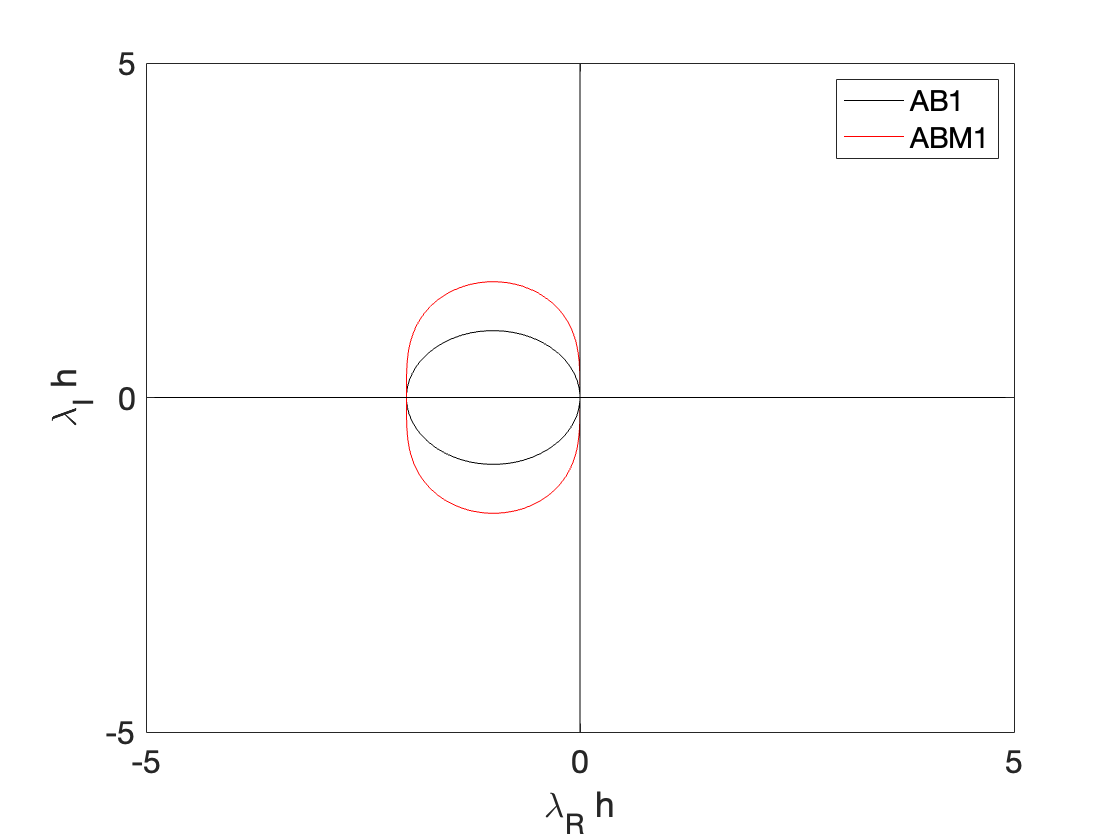
\includegraphics[width=0.5\textwidth]{p1_1.png}
%  \caption{Linear stability diagram after the first corretor step. }
%  \label{fig1_1}
%\end{figure}
\end{document}